
\documentclass{article}
\usepackage{multicol}
\usepackage{graphicx}
\usepackage{float}
\usepackage{sectsty}
\usepackage{titlesec}
\titlespacing*{\section}
{0pc}{*3}{*2}[3pc]
\pagenumbering{gobble}
\sectionfont{\fontsize{11}{12}\selectfont}
\usepackage[margin=1.5cm]{geometry}

\begin{document}
  \begin{multicols}{2}
    \begin{center}

    \large
    \textbf{Pre-Processing and Layout Analysis for Offline Handwriting recognition}

    \normalsize
      Pitk{\"a}nen Perttu

      Academic advisors: Kawamata Masayuki, Abe Masahide

      Kawamata/Abe laboratory

      Department of Electronic Engineering
      \end{center}

      \section*{Introduction}
        Handwriting recognition is a process to extract the textual information from image containing handwritten characters, into computer readable form. This is done by applying various image processing and classification methods to the input image. In this research experients are made with varying methods regarding preprocessing and layout analysis phases. For quick development the implementation is done with MATLAB programming language and tools including image processing toolbox.

      	In preprocessing stage the quality of image is enhanced and the area of text is located.  The feature extraction stage captures the distinctive characteristics of the digitized characters for recognition. Lastly in during the classification stage the feature vectors are used with machine learning to identify the  words.

      \section*{Methods}
        Firstly as much as possible noise is to be removed. For this purpose adaptive Wiener filter is used. The adaptive filter can recognize the amount of variance and adjust the smoothing according to it.

      	After noise removal the image must be binarized. This is one of the most crucial parts of the preprocessing as information can be lost if it's not done properly. For this purpose the Sauvola binarization algorithm was chosen as it was designed for document binarization purposes.

      	For detecting text regions from the image the stroke width variation is observed. The image objects having only a little amount of variance in stroke width can be considered text region compared to high variance objects such as photographs or drawings. The objects are discarded if they have larger variance than pre-defined threshold.

        Afterwards the process proceeds to layout analysis phase and in this case line detection process. The implemented method was proposed by Louloudis et.al. and it provides a sophisticated approach to detect handwritten text lines even if they overlap each other. This is done with so called Hough transform mapping.

        \begin{figure}[H]
          \centering
          \includegraphics[natwidth=555,natheight=555,scale=0.6]{hough_space.png}
          \caption{$\theta$ and $\rho$ are be used to describe a line in Cartesian space. The current line is marked in red. \label{fig:houghspace2}}
        \end{figure}

        Hough transform is used to find lines in cartesian space using data points as input. In this case the data points are multiple block centroids aquired by splitting the component into smaller sections. The Hough transform results in accumulator array that shows which $\theta$ and $\rho$ values realize most lines. When a line is found all components assigned to it are removed from the accumulator array and the process is continued until no new lines can be found. Afterwards the smallest objects which represent accents and punctuation marks are assigned to nearest line and the largest objects are split into smaller objects if they overlap multiple lines.

        \begin{figure}[H]
          \centering
          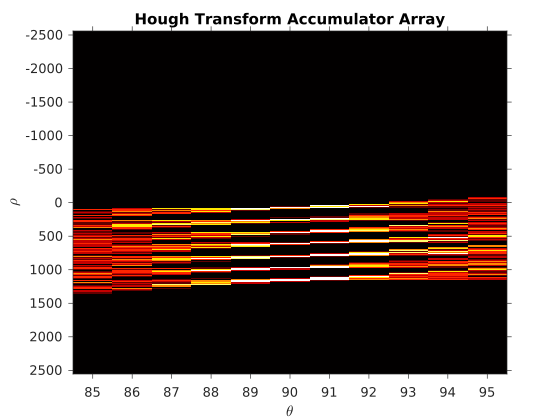
\includegraphics[natwidth=560,natheight=420,scale=0.3]{hough_accArr_a01-000u.png}
          \caption{Seven lines can be detected with this accumulator array.\label{fig:houghacc2}}
        \end{figure}

        \section*{Evaluation}
          Several tests were conducted in order to gain insight on which methods work best with which parameter values and what kind of effect the changes have to the output. The methods were tested with 100 images from handwriting database containing different English language texts by different writers.

          Tests were conducted for the preprocessing methods Wiener filtering and Sauvola binarization algorithm. For layout analysis phase the stroke width variance threshold and several constant parameters for Hough transform mapping were evaluated. The tests used the number of detected lines as the metric to measure the accuracy of the system compared to the true amount of lines.

        \section*{Conclusions}
          Aforementioned parameters were tested and their effect was studied. The binarization parameters had a significant effect on the recognition process. However the Hough transform mapping is only dependant on the paramters that affected the initial line detection from the accumulator array and the other parameters didn't have noticeable effect on the output. Some constraints regarding the line detection were found, such as the method can detect lines from single column text.

          As for future work the word detection should be implemented. At this point the system is only capable of recognizing individual lines of handwritten text. The feature extraction and classification phases should also be implemented for the whole recognition process to be complete. This would allow more accurate evaluation of the whole system.

   \end{multicols}
\end{document}
